\documentclass[a4paper]{report}
\usepackage[utf8]{inputenc}
\usepackage[english]{babel}
\usepackage{hyperref}
\usepackage{a4wide}
\usepackage{pmboxdraw}
\usepackage{minted}
\hypersetup{pdftitle={Elevado número de fontes de luz},
pdfauthor={José Ferreira, Jorge Mota},
colorlinks=true,
urlcolor=blue,
linkcolor=black}
\usepackage{subcaption}
\usepackage{listings}
\usepackage{booktabs}
\usepackage{multirow}
\usepackage{appendix}
\usepackage{tikz}
\usepackage{authblk}
\usepackage{bashful}
\usepackage{verbatim}
\usepackage{amssymb}
\usepackage{multirow}
\usepackage{mwe}
\usepackage{float}
\usepackage{graphics}
\usetikzlibrary{positioning,automata,decorations.markings}

\begin{document}

\title{Visualização e Iluminação II\\Elevado número de fontes de luz}
\author{José Ferreira (A83683), Jorge Mota (A85272)}
\date{\today}

\begin{center}
    \begin{minipage}{0.75\linewidth}
        \centering
        
\includegraphics[width=0.4\textwidth]{images/eng.jpeg}\par\vspace{1cm}
        \vspace{1.5cm}
        \href{https://www.uminho.pt/PT}
        {\color{black}{\scshape\LARGE Universidade do Minho}} \par
        \vspace{1cm}
        \href{https://www.di.uminho.pt/}
        {\color{black}{\scshape\Large Departamento de Informática}} \par
        \vspace{1.5cm}
        \maketitle
    \end{minipage}
\end{center}

\tableofcontents

\pagebreak
\chapter{Introdução}
%%%%%%%%%%%%%%%%%%%%%%%%%%%%%%%%%%%%%%%%%%%%%%%%%%%%%%%%%%%%%%%%%%%%%%%%%%%%%%%%
Iluminacao e algo fundamental para a criação de ambientes simulados em
computador que sejam realistas e visualmente agradáveis. 
Para simular de forma realista o caminho que e necessário computar para cada
ponte de cada superfície quais são as luzes que afectam a sua aparência. Desta
forma,  com o aumento das luzes numa dada cena a complexidade de a computar
também tem tendência a aumentar.\\
Visto que tal e completamente impraticável existem soluces que tentam mitigar
este problema.\\
Ao longo deste relatório iremos explorar e comparar diversas soluções
desenvolvidas.

\chapter{Implementação}
%%%%%%%%%%%%%%%%%%%%%%%%%%%%%%%%%%%%%%%%%%%%%%%%%%%%%%%%%%%%%%%%%%%%%%%%%%%%%%%%
O nosso objetivo principal consiste em encontrar um equilíbrio na renderização
das luzes num ponto, de forma a \underline{diminuir o custo de computação} e
\underline{diminuir o tempo de convergência}.

Primeiro começamos por obter métricas de performance com base no código
disponibilizado no Tutorial 4. Este tutorial aplica o \textit{shading} de todas
as luzes a todos os pontos, tendo uma solução O(n), sendo \textbf{n} o numero de
luzes totais na cena.

\begin{figure}[H]
    \centering
    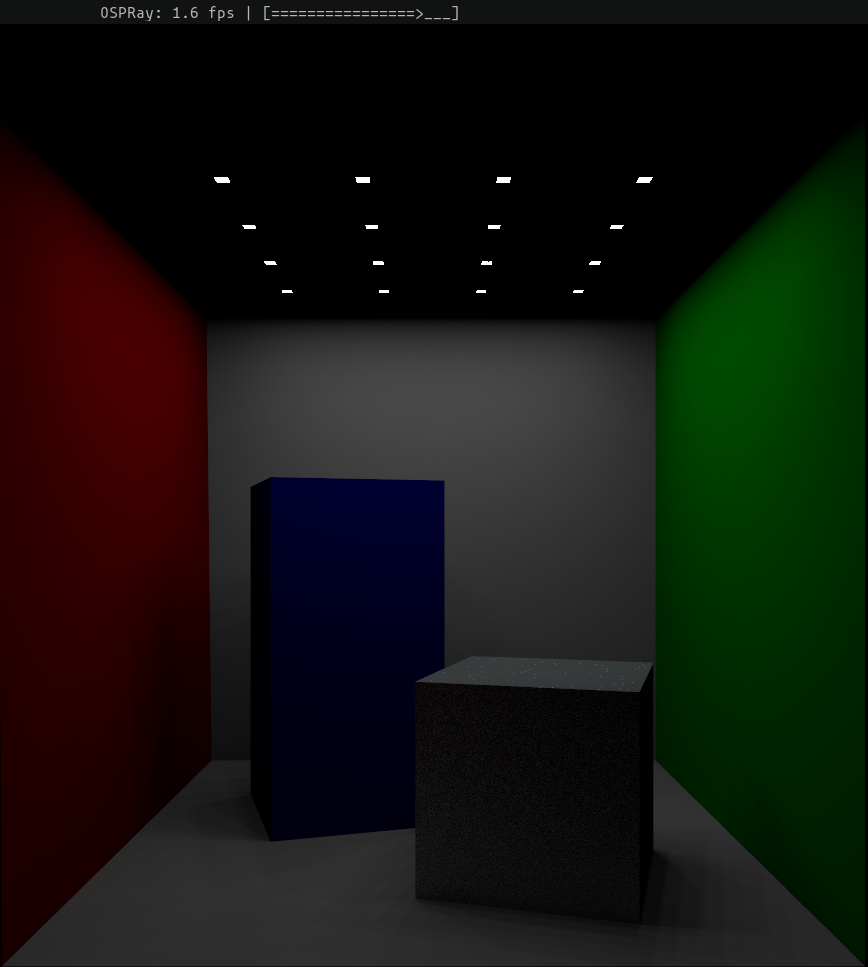
\includegraphics[height=8.cm]{images/test_1.png}
    \caption{Amostragem de todas as luzes (\texttt{$\sim$1.5 FPS})}
\end{figure}

Esta foi a solução original que utilizamos como base para
comparar os resultados das mudanças que fizemos.

\pagebreak

\section{Aumentar o número de luzes}
%%%%%%%%%%%%%%%%%%%%%%%%%%%%%%%%%%%%%%%%%%%%%%%%%%%%%%%%%%%%%%%%%%%%%%%%%%%%%%%%

Para que o cenário da Cornell Box seja aplicável para o nosso caso de estudo é
necessário primeiro aumentar o número de luzes deste. Para isso inserimos novas
luzes ao longo do teto, compondo o código de forma a podermos facilmente aumentar
o número de luzes a qualquer momento.

\begin{figure}[H]
    \centering
    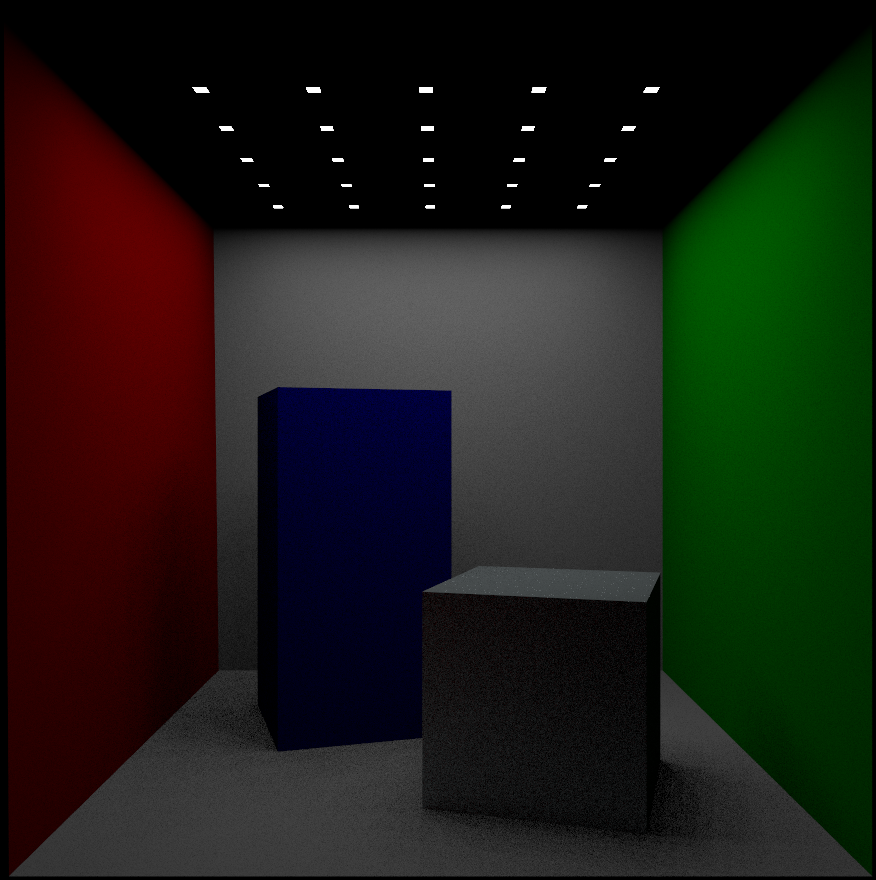
\includegraphics[height=4.5cm]{images/5_lights.png}
    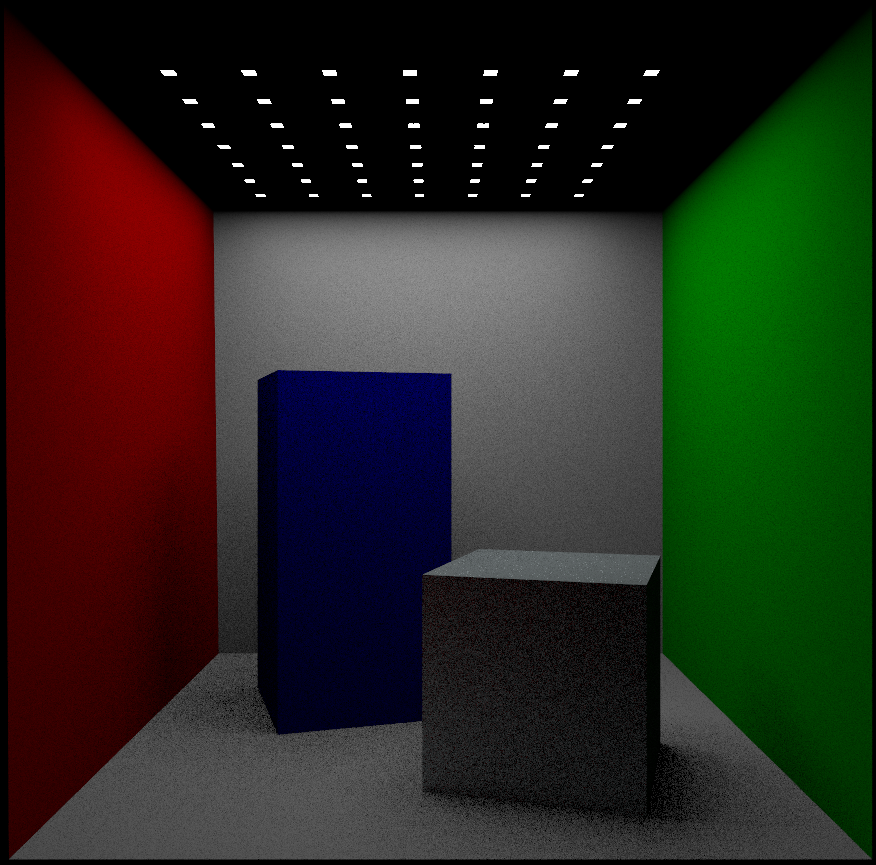
\includegraphics[height=4.5cm]{images/7_lights.png}
    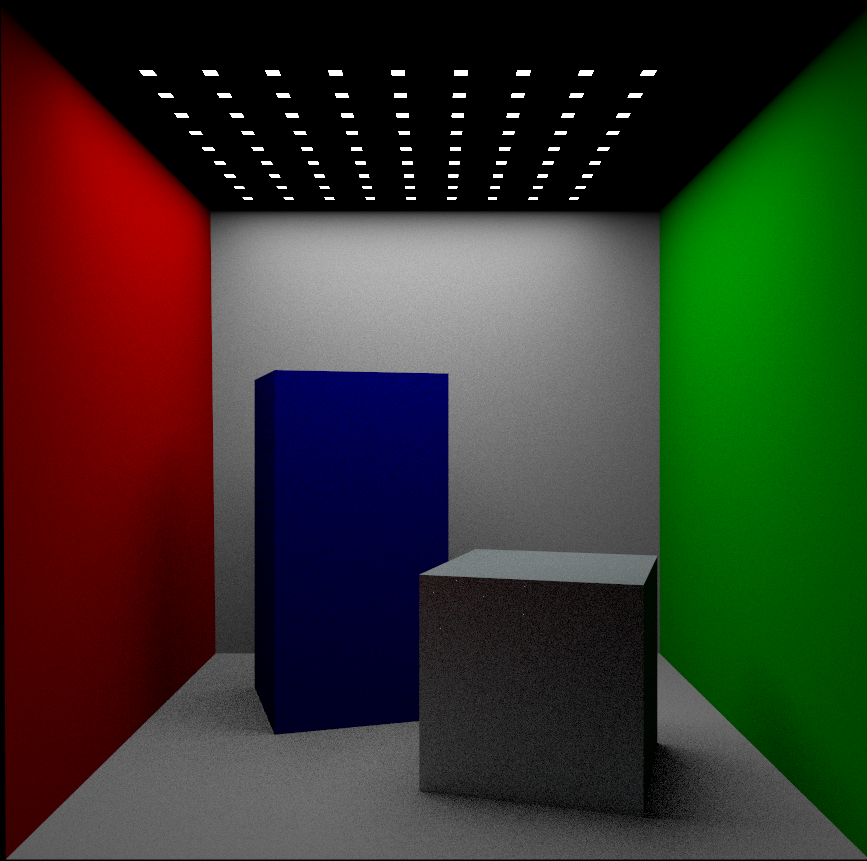
\includegraphics[height=4.5cm]{images/9_lights.png}
    \caption{luzes (5x5, 7x7, 9x9)}
\end{figure}

\section{Amostragem de luzes de forma uniforme}
%%%%%%%%%%%%%%%%%%%%%%%%%%%%%%%%%%%%%%%%%%%%%%%%%%%%%%%%%%%%%%%%%%%%%%%%%%%%%%%%

Uma possível solução para diminuir o custo de computação significativamente é
selecionar de forma aleatória com uma distribuicao uniforme uma luz e dividir a
radiância emitida pela luz (se não ocludida) pela probabilidade de cada luz ser
selecionada.

\begin{figure}[H]
    \centering
    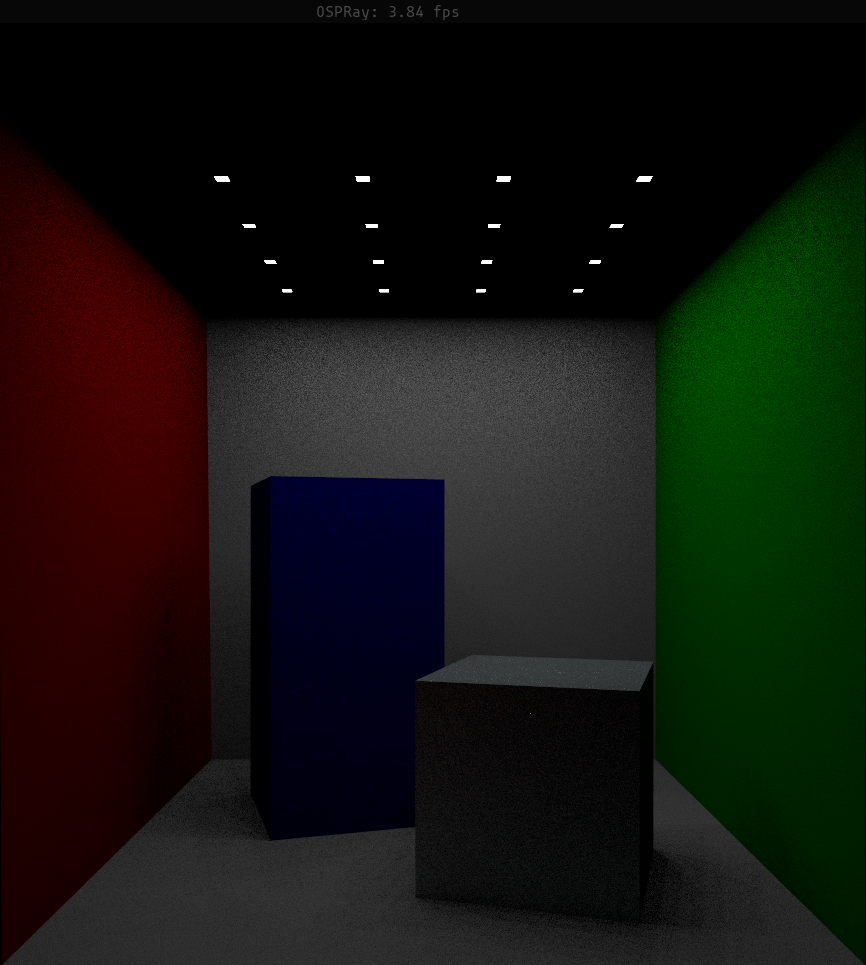
\includegraphics[width=0.6\textwidth]{images/test_2.png}
    \caption{Amostragem uniforme (\texttt{$\sim$3.8 FPS})}
\end{figure}

A performance do path tracer melhorou significativamente de $\sim$1.5FPS para
$\sim$3.8FPS. No entanto,  podemos notar algum aumento do ruído presente na
imagem, nomeadamente na parede e no chão. Tal deve-se ao facto de como escolhemos
de forma aleatoriamente uniforme a luz que vai dar \textit{shade} a um certo ponto
tem igual probabilidade de escolher qualquer luz,  o que significa que não há
qualquer noção de quais as luzes influenciam mais aquele ponto. Tal também leva a
um aumento do tempo de convergência.

\section{Amostragem de luzes de forma pesada}
%%%%%%%%%%%%%%%%%%%%%%%%%%%%%%%%%%%%%%%%%%%%%%%%%%%%%%%%%%%%%%%%%%%%%%%%%%%%%%%%

Finalmente chegamos à solução final que produz resultados relevantes para manter
uma quantidade de ruído reduzida, e reduzir o tempo de computação.

Esta solução, reutiliza o modo de amostragem uniforme, mas as probabilidades de
cada luz são reflectidas pelo grau de contribuição que essa luz produz para um
certo ponto.

Este método é implementado a partir de dois vetores com tamanho \texttt{numLights}
(\texttt{lights\_pdf}, \texttt{lights\_cdf}) que têm a probabilidade de cada luz e
a probabilidade acumulada. É amostrado um número de 0 a 1 e utiliza-se a
probabilidade acumulada para saber qual das foi seleccionada, de seguida
calcula-se a radiância emitida e divide-se pela respectiva probabilidade para
aquela luz. 

\begin{figure}[H]
    \centering
    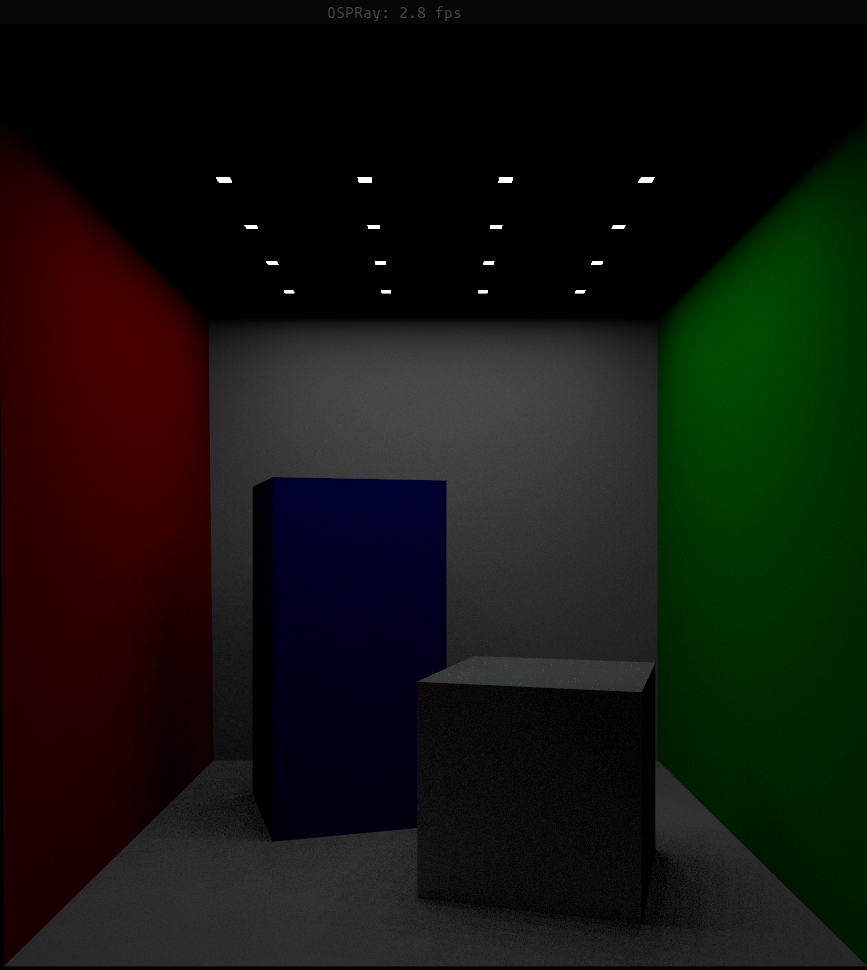
\includegraphics[height=8.cm]{images/test_3.png}
    \caption{Amostragem pesada de uma luz (\texttt{$\sim$3.0 FPS})}
\end{figure}

Como podemos observar os resultados mostram que há muito menos ruído, enquanto
que se mantém a performance melhor que a solução do Tutorial 4.

\end{document}
